\chapter{Incorporating land-cover changes between 1992 and 2015 into biodiversity projections }
%\addcontentsline{toc}{chapter}{Chapter 4}
%\markboth{}{Incorporating land-cover changes between 1992 and 2015 into biodiversity projections }
\label{C04}

Changes in global land cover are important factors that determine past and present biodiversity projections. It has been proposed that attributes of land-cover change, such as the time passed or the sequence in land cover \textendash\ \ie\ from forest to agriculture \textendash\ likely affect local biodiversity differently. Additionally, attributes of land-cover change may have lasting impacts on local biodiversity and thus need to be considered while assessing biodiversity change. Yet, the impacts of attributes of past land-cover change on local biodiversity have not been fully determined globally and most existing biodiversity projections remain largely uninformed of past land-cover change. Here, we combine time series of annual land cover from the period 1992 to 2015 with data of local biodiversity globally. Using hierarchical models comparing sites with and without a land-cover change in the past, we ask whether biodiversity differences vary with the time passed or the sequence after a land-cover change occurred and how this affects global and national biodiversity projections. Overall, we found local biodiversity to be consistently lower in sites with a past land-cover change. However, with increasing time passed after land-cover change local biodiversity recovered to levels comparable to unchanged sites. Furthermore, depending on the land-cover sequence, we observed either increases or decreases in local biodiversity and we demonstrated how a consideration of past land-cover change affects global and national biodiversity projections, especially so in tropical and economically developing countries. Our findings suggest that most global and national biodiversity projections overestimate biodiversity change and that lasting influences of past land-cover change need to be taken into account.

\section{Introduction}
\label{C04_01}

The terrestrial surface of the Earth is shaped by natural and anthropogenic processes \citep{Foley2005}. The outcomes of these processes alter soil, plant and human structures, which collectively define terrestrial land cover \citep{DiGregorio2000,Lambin2006}. Land cover \textendash\ quantified as either continuous or categorical estimate of the Earth's land surface conditions \textendash\ is commonly derived from remotely-sensed spectral measurements with many studies having mapped the distribution of land-cover categories globally \citep{DeFries1994,Hansen2000,Tuanmu2014,Grekousis2015}. Knowledge of land-cover change is important to help understand and create future projections and scenarios of biodiversity change \citep{Harfoot2014,Titeux2016,Kehoe2017a}. Yet only few temporally consistent estimates of land-cover change, with exception of vegetation \citep{Hansen2013,Song2018} or water-covered areas \citep{Pekel2016}, are publicly available at the global scale. 

Quantifying change in remotely-sensed land cover is challenging. For continuous representations of land cover, remotely-sensed changes are commonly detected by exploiting differences in timing, amplitude and direction of remotely-sensed spectral measurements \citep{Coppin2004,Lhermitte2011,Zhu2017}. There have been initial attempts to incorporate land-cover changes detected from these differences into categorical land-cover maps \citep{Zhu2014,Hermosilla2018}, but the majority of land-cover maps remain uninformed of preceding land cover. Quantifying temporal change in categorical representations of land cover has been problematic because of inconsistencies in thematic resolution that lead to unrealistic estimates of land-cover change \citep{VERBURG2011,Cardille2016,Abercrombie2016}. A new generation of temporally consistent time series of land cover \citep{ESA2017,Hermosilla2018,Nowosad2018,Sulla-Menashe2019} are beginning to emerge that allow the investigation of land-cover change globally and its impacts on biodiversity.

Biodiversity is impacted by past and current differences in land cover \citep{Newbold2015,Newbold2016a,Jung2018}. Local species richness has been estimated to be up to 31\% lower globally in the most anthropogenically-modified land compared to “primary vegetation” sites \citep{Newbold2015}. However most previous global studies have considered only differences in land use and/or land cover at the time of biodiversity sampling \citep{Gibson2011,Murphy2014,Newbold2015}, thus ignoring lasting influences of past changes in land cover. There is evidence that the occurrence and abundance of species is not only determined by differences in current but also past land cover (Chapter \ref{C03}) through so called ‘biotic lag’ effects, such as ecological memory effects \citep{Ogle2015} or extinction debts \citep{Kuussaari2009}. The impacts of past land-cover change on biodiversity likely depend on certain attributes such as magnitude and time passed since land-cover change \citep[Chapter \ref{C03}, ][]{Martin2013,Watson2014,Fu2017} or the sequences of land-cover \citep{Watson2014,Nowosad2018}. 

Land-cover change causes varying sequences of land cover \citep{Nowosad2018}, which often have differing impacts on local biodiversity \citep{Foster2003}. \cite{Bremer2010} reported an average loss of species richness globally for land changing from grass- or shrubland to forest cover, but not for land changing from secondary vegetation to forest cover. Meanwhile, biodiversity in secondary vegetation has been shown to recover more quickly if land was previously covered by grassland rather than agriculture \citep{Dyer2010}, although among taxonomic groups, especially plant diversity, abundance and growth have been shown to be influenced by lasting influences of an agricultural past \citep{Chazdon2003,Fraterrigo2006,DeFrenne2010,Perring2018}. Other studies have highlighted the lasting effect that changes in forest \citep{Gonzalez2016} or wetland cover \citep{Halstead2014} might have on biodiversity. While these studies suggest that land-cover sequences need to be considered for explaining differences in local biodiversity, little is known about the influence of land-cover sequences across taxonomic groups and at global and national scales, which could affect projections of biodiversity.

To guide decision making, projections of global and national biodiversity change are often useful to inform policy \citep{Pereira2010,Visconti2014}. Biodiversity projections can be used to create scenarios of biodiversity change in response to pressures such as land change \citep{Newbold2015,Newbold2016a,Titeux2016}, which can inform science-policy platforms \citep{Harfoot2014,Visconti2014,Purvis2018} like the Intergovernmental Platform on Biodiversity and Ecosystem Services (IPBES). However most existing biodiversity projections ignore lasting effects of past land-cover change. This is especially problematic for tropical, developing nations, where much land has been converted from forest to agriculture or pasture covered land in recent decades \citep{Curtis2018} and that are recognized as global biodiversity hotspots \citep{Brooks2002,Laurance2014b}. Under a business-as-usual scenario of future biodiversity change, especially less economically developed countries will suffer the greatest losses in local biodiversity \citep{Newbold2015,Visconti2014}, however these projections might \textendash\ depending on attributes of land-cover change \textendash\ over- or underestimate impacts on biodiversity.

The overall aim of this study is to investigate (\textit{i}) how local biodiversity is impacted by a land-cover change in the past as derived from a global remotely-sensed land cover product, (\textit{ii}) if impacts on local biodiversity differ with attributes of land-cover change such as differing sequences of land cover or time passed \citep{Watson2014}, and (\textit{iii}) how particularly differing sequences of land cover affect global and national biodiversity projections. Overall, this study adds to our knowledge of how attributes of land-cover change affect local biodiversity and demonstrates how these attributes can be incorporated into global and national biodiversity projections.   

\section{Methods}
\label{C04_02}
\subsection{Species assemblage data}
\label{C04_0201}

The local biodiversity data were derived from a snapshot (obtained Feb 2016) of the Projecting Responses of Ecological Diversity In Changing Terrestrial Systems (PREDICTS) database which collated data on species’ presence and abundance at sampled ‘sites’ from published ‘studies’ \citep{Hudson2016}. Each PREDICTS site has associated spatial coordinates \textendash\ usually obtained from the text or author of a published study \textendash\ and a record of when and how long biodiversity sampling took place. Species assemblages in the PREDICTS database were sampled at various sampling extents (maximum linear extent, MLE) which are defined by methodology and taxonomic group \citep{Hudson2014}. To link local biodiversity with remotely-sensed land cover data (see \ref{C04_0202}), we used the spatial coordinates of all sites provided by the PREDICTS database as for the majority of sites, the MLE is fully contained (median MLE = $40 \pm 56.49$ MAD) within the used grid cell size (\textasciitilde 300m, see methods \ref{C04_0202}).   

Similar to previous analyses using the same data (\eg Chapter \ref{C02} in this thesis), we calculated several biodiversity measures including the total number of species, individuals and the species assemblage evenness at the site level. We calculated local species richness and \textendash\ where data on species abundance was available \textendash\ the total abundance for each PREDICTS site. For those studies in PREDICTS with differing sampling effort among sites we corrected measures of total abundance by assuming that total abundance increases linearly with sampling effort \citep{Newbold2014b,Newbold2015}. As a measure of assemblage evenness, we calculated the probability of an interspecific encounter (PIE), which quantifies the probability of two individuals randomly chosen from an assemblage representing different species \citep{Hurlbert1971}. 

\subsection{Annual land cover data}
\label{C04_0202}

We used estimates of land cover (LC) from a global dataset produced by the European Space Agency Climate Change Initiative \citep[][ver. 2.0.7 obtained from \href{http://maps.elie.ucl.ac.be/CCI}{http://maps.elie.ucl.ac.be/CCI} ]{ESA2017}. The ESA LC product quantifies global land cover annually from 1992 to 2015 with a spatial resolution of \textasciitilde 300m \citep{ESA2017} and a thematic resolution of 22 land-cover categories \citep[75.38\% global accuracy, ][]{ESA2017} at two different hierarchies (level 1 and 2), that follow the Land Cover Classification System \citep[LCCS, ][]{DiGregorio2000} of the United Nations Food and Agriculture Organization. Compared to many existing LC products \citep{Grekousis2015}, we used the ESA LC product because of its comparably long availability (1992 to 2015) and ability to detect land-cover changes \citep{ESA2017}. However the change detection algorithm in the ESA LC product does not come without caveats as only land-cover changes persistent over at least two years \textendash\ in contrast to "short-lived" land changes \citep{Lambin2006} \textendash\ are detected. Furthermore abrupt land-cover changes (such as forest to agriculture) tend to be better captured than gradual land changes \citep{ESA2017} and in the years 2014 and 2015 only changes in forest cover could be reliably detected \citep{ESA2017}. Despite these caveats, estimates of land-cover change from the ESA LC product have good agreement with other, independently developed, land-cover change products \citep{Li2018}.

For this study, we extracted for each PREDICTS site the land-cover sequence from the ESA LC product (Figure \ref{F04_01}\textbf{c}-\textbf{d}). Before extracting these sequences, we reclassified the original ESA LC level 2 categories (22 categories based on the LCCS) to the level 1 hierarchy (10 LC categories, namely: forest, shrubland, grassland, sparse vegetation, agriculture, urban, bare area, wetland, water, and other) to reduce inaccuracies caused by misclassifications and because temporal changes between ESA LC level 2 categories can be poorly captured \citep{ESA2017}. PREDICTS sites where the extracted ESA LC level 1 categories indicated “water” or “other” (such as snow and ice) at the start of biodiversity sampling were removed from further analyses (N = 262 sites). In this study we focussed only on sequences of land cover with a single land-cover change before biodiversity sampling as two or more land-cover changes were rarely observed globally (Figure \ref{F04_01}\textbf{a}) and did only occur at two PREDICTS sites, which were excluded from further analyses.  

% ---------------- Figure 1 --------------------- %
\begin{figure}[htb]
\centering
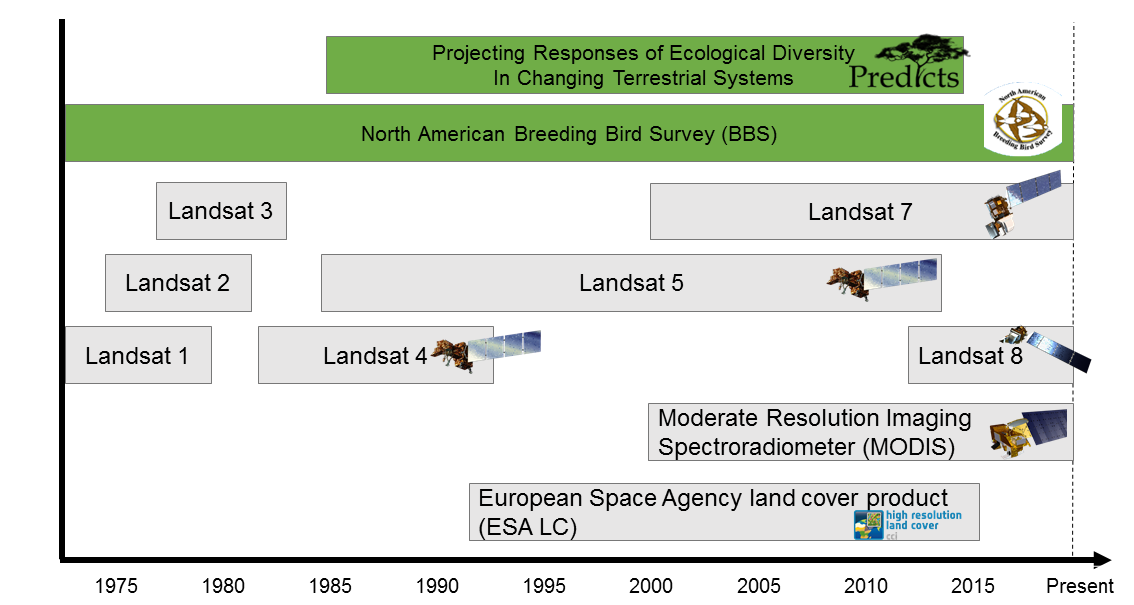
\includegraphics[width=1\textwidth]{chapter4/F01}
\caption{ (\textbf{a}) Global map depicting the grid cells of the ESA LC product that had $\geq 1$ land-cover change (red) in the period 1992 to 2015. Inset maps focus \textendash\ from left to right \textendash\ on the deforestation in the eastern Amazon basin, expanding soy plantations in Paraguay as well as shrubland loss in south east Australia. Map is projected in an equal-area Mollweide projection (\textbf{b}) Mean proportion (in \%) of land with a land-cover change (red) in the period 1992 to 2015 averaged per 1\textdegree\ of latitude. (\textbf{c}) Example land cover maps of the past and at the time of biodiversity sampling for a single study. Black symbols indicate sites with (diamond) and without (circle) land-cover change. (\textbf{d}) Flow diagram showing the sequence of land cover of all PREDICTS sites with a past land-cover change. Colours as in \textbf{c}.  }
\label{F04_01}
\end{figure}
% -------------------------------------------- %

\subsection{Analyses}
\label{C04_0203}

The statistical analysis for this study had two main aims. First, we aimed to quantify whether biodiversity measures were different at sites with a past land-cover change compared to sites without any land-cover change in the period 1992 to the start of biodiversity sampling. To do so, we fitted generalized linear mixed effects models (GLMMs) using Poisson distributed errors for species richness and a Gaussian error distribution for total abundance (log10 transformed) and the probability of an interspecific encounter (PIE, asin-squareroot transformed). Following previous studies \citep{Newbold2015,Jung2016} all models included the study identity and a spatial block of sampling design and additionally the ESA LC category at the time of biodiversity sampling as random intercept. We fitted separate GLMMs to assess the difference in local biodiversity measures between sites with and without (\textit{i}) a past land-cover change overall, (\textit{ii}) a categorical representation of the time passed since a land-cover change occurred (unchanged, \ie $0$ years, or $\leq$ $5$, $5-10$, >$10$ years), (\textit{iii}) distinguishing sites with and without a past land-cover change by their land-cover sequence, for which we fitted separate GLMMs for each ESA LC category at the time of biodiversity sampling using the extracted sequence of land-cover (those with at least 10 sites to ensure robustness of coefficients) categories as fixed effect (Figure \ref{F04_01}\textbf{b}). Lastly (\textit{iv}) we fitted a GLMM using the ESA LC categories at the time of biodiversity sampling and as interacting covariate, human population density data from the global human settlement (GHS) project \citep{Pesaresi2013,Pesaresi2016} as coarse proxy for anthropogenic use. We used data from the GHS project as it is available at a spatial (\textasciitilde 250m) and temporal (1975-2015) resolution that matches the resolution of the ESA LC data. All GLMMs were fitted using the ‘lme4’ package \citep[ver. 1.1-18-1,][]{lme4} in R \citep[ver. 3.5, ][]{RTeam2014}.

Second, we constructed global and national projections of biodiversity. We used the model described above (\textit{iv}) to project the mean coefficients of local biodiversity onto the global ESA LC map for the year 2015 only, which we resampled to \textasciitilde3 x 3 km spatial resolution by assigning the most dominant (‘modal’) LC value to each grid cell. All predicted biodiversity estimates were transformed relative to the predicted biodiversity estimates of a ‘forest’ site with zero human population density in the year 2015 \citep{Newbold2015}. Biodiversity sampling in the majority of PREDICTS sites (96.2\%) occurred between 2000 and 2013 and from the ESA LC maps of the years 2000 and 2015 we constructed a new global map for the year 2015 with each grid cell set to a unique categorical code of the sequence of land-cover (using Cantor’s pairing function). For each separate model (see \textit{iii} above) and unique sequence of land-cover categories a new spatial projection was created for those grid cells with the respective sequence. We then added (to the mean coefficients) those separate spatial projections to the projection of the global mean difference in local biodiversity for the year 2015 (see above), thus “updating” the projected difference in only those grid cells where a past land-cover change has occurred (see Appendix Figure \ref{SI04_01} for a schematic). Some land-cover sequences were not available among PREDICTS sites and here we used the global average impact (see model \textit{i}) in place of no better data available. Because of data limitations, we were also not able to investigate the impact of interactions between land-cover sequences and time passed on local biodiversity. Globally each grid cell has a different baseline level of local biodiversity \textendash\ \eg\ deserts being less species richness than shrublands \textendash\ and we followed \cite{Newbold2015} by weighting all grid cells using either a normalized global layer of terrestrial vertebrate diversity \citep[summed range-of-occurrence maps for bird, mammal and amphibian species,][]{NatureServe2012,IUCN2016a} for species richness or a layer of global photosynthetic activity (average photosynthetic activity as measured by MODIS NDVI in the period 2000-2015) for total abundance and assemblage evenness \citep{Newbold2015}. 

Global biodiversity projections were visualized in a way that emphasises model uncertainty by supressing predicted biodiversity estimates with large uncertainty \citep{Correll2018}. We refitted the GLMM models using the ‘mgcv’ package \citep[ver. 1.8-24, ][]{Wood2011} because of it's ability to obtain estimates of prediction uncertainty for hierarchical models. For each grid cell we predicted the standard error from the Bayesian posterior covariance matrix of the ‘mgcv’ model \citep{Wood2011} and used it to calculate the absolute error in the predicted difference of local biodiversity (known as mean absolute error or MAE). To use the MAE for visual suppression of uncertain projected biodiversity estimates, we excluded the 1\% lowest and highest MAE estimates and furthermore normalized ($ \frac{(MAE - min(MAE) )}{(max(MAE) - min(MAE))} $) the MAE globally. To assess whether accounting for past land-cover sequences affects national biodiversity projections, we calculated the area-weighted relative mean difference in biodiversity at the national scale compared to a spatial projection where past land-cover changes are not taken into account ($\frac{x_{Sequence} -x_{without} }{|x_{without}|}$, where $x$ is the mean area-weighted predicted national difference in biodiversity). We differentiated countries into groups of high (black), middle (orange) or low (blue) income (according to \href{http://data.un.org}{http://data.un.org}) and assessed differences between those groups using ordinary analysis of variance (ANOVA) tests.

\section{Results}
\label{C04_03}

Across all sites in the PREDICTS database, 1326 sites had a single land-cover change in the years before biodiversity sampling compared to 13696 sites without any change (number of studies: 238). The greatest number of PREDICTS sites with a past land-cover change were forest covered (552), followed by agriculture (442) and urban covered (126) sites (Appendix Figure \ref{SI04_02}). Overall, sites with a past land-cover change had on average 5.3\% ($\pm$ 0.01 SE, p < 0.001) fewer species, 6.1\% ($\pm$ 0.03 SE, p < 0.001) fewer individuals and were 1.1\% ($\pm$ 0.01 SE, p = 0.217) less even compared to a site without a past land-cover change. With increasing time passed after a land-cover change occurred, local species richness and total abundance recovered to levels comparable to unchanged sites (Figure \ref{F04_02}). If a land-cover change occurred in the five years before biodiversity sampling, sites had on average 5.6\% ($\pm$ 0.01 SE, p < 0.001) fewer species and 8.5\% ($\pm$ 0.04 SE, p < 0.05) fewer individuals than sites without a land-cover change in the past. Compared to unchanged sites, assemblage evenness was not significantly different (1.6\% $\pm$ 0.01 SE, ns) for sites with a land-cover change less than 5 years ago but was significantly lower (4.4\% $\pm$ 0.01, p < 0.01) after 5 to 10 years had passed. 

% ---------------- Figure 2 --------------------- %
\clearpage
%\begin{figure}[!h]
\begin{wrapfigure}{r}{.5\textwidth}
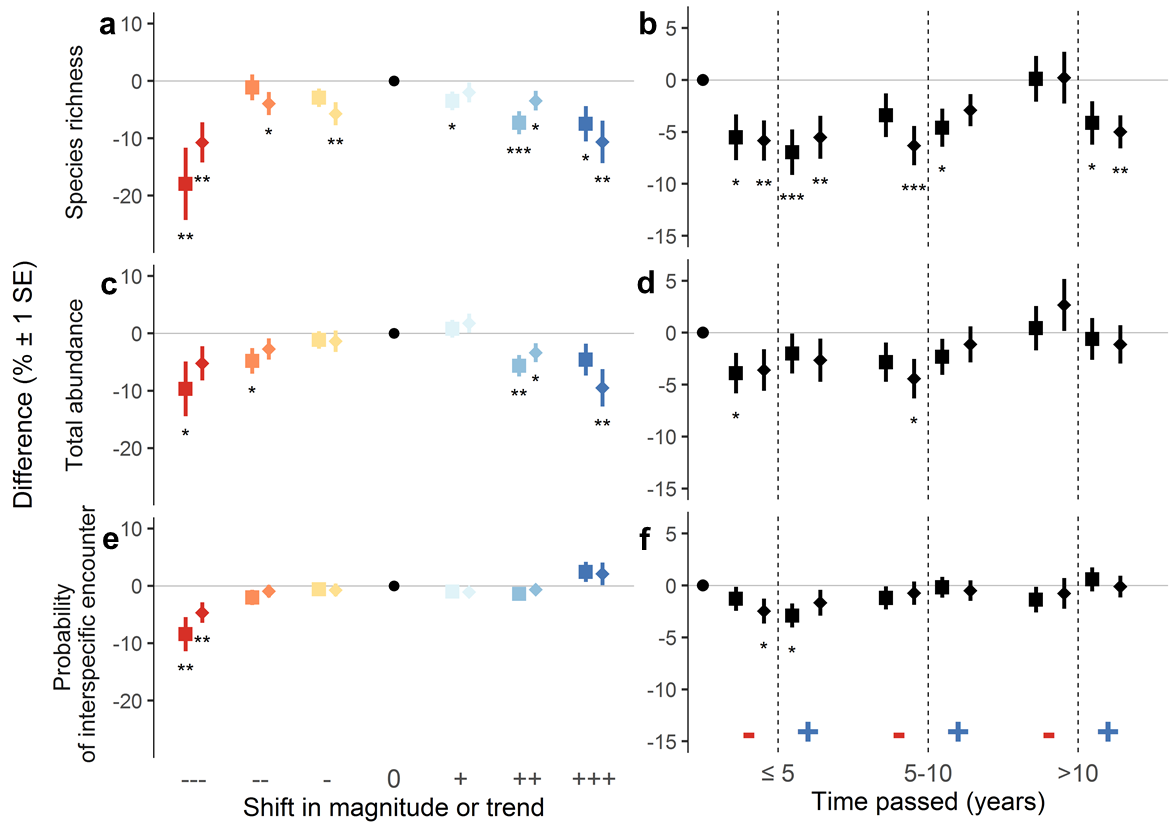
\includegraphics[width=.5\textwidth]{chapter4/F02}
\caption{ Difference in local biodiversity measures between sites without ($0$) and sites with a past land-cover change that occurred $\leq$ 5 years, > 5-10 or over 10 years ago. The error bars show the predicted standard error and stars (*) indicate whether the difference was statistically significant (p < 0.05). The total number of sites is indicated. }
\label{F04_02}
\end{wrapfigure}
%\end{figure}
% -------------------------------------------- %

Local biodiversity varied between sites with and without a past land-cover change depending on past land-cover sequences (Figure \ref{F04_03}). The number of species (11.4\% $\pm$ 4 SE) and individuals (13.4\% $\pm$ 12.9 SE) of forest sites was lower if the site had been shrub covered before biodiversity sampling compared to forest sites without a land-cover change in the past (Figure \ref{F04_03}\textbf{a}), while the number of species was higher (17.4\% $\pm$ 5.51 SE) if the preceding land cover had been grassland. More species (10.83\% $\pm$ 5.51 SE) and individuals (26.1\% $\pm$ 15.1 SE) were found in previously forest covered sites compared to shrubland sites without a past land-cover change (Figure \ref{F04_03}\textbf{b}). The number of species and individuals in agricultural sites was lower if the preceding land cover was forest (8.81\% $\pm$ 2.1 SE for species and 6.93\% $\pm$ 6.9 SE for individuals) or shrubland (23.93\% $\pm$ 3.9 SE and 35.8\% $\pm$ 18.4 SE) compared to sites without a land-cover change in the past (Figure \ref{F04_03}\textbf{e}). Sites with urban land cover had in most cases higher number of species, individuals and assemblage evenness (up to 80.2\% $\pm$ 30 SE for abundance in agriculture, Figure \ref{F04_03}\textbf{f}) compared to urban sites without a past land-cover change, with only species assemblages in previously agricultural sites being less even (Figure \ref{F04_03}\textbf{f}).

% ---------------- Figure 3 --------------------- %
\begin{figure}[!hb]
\centering
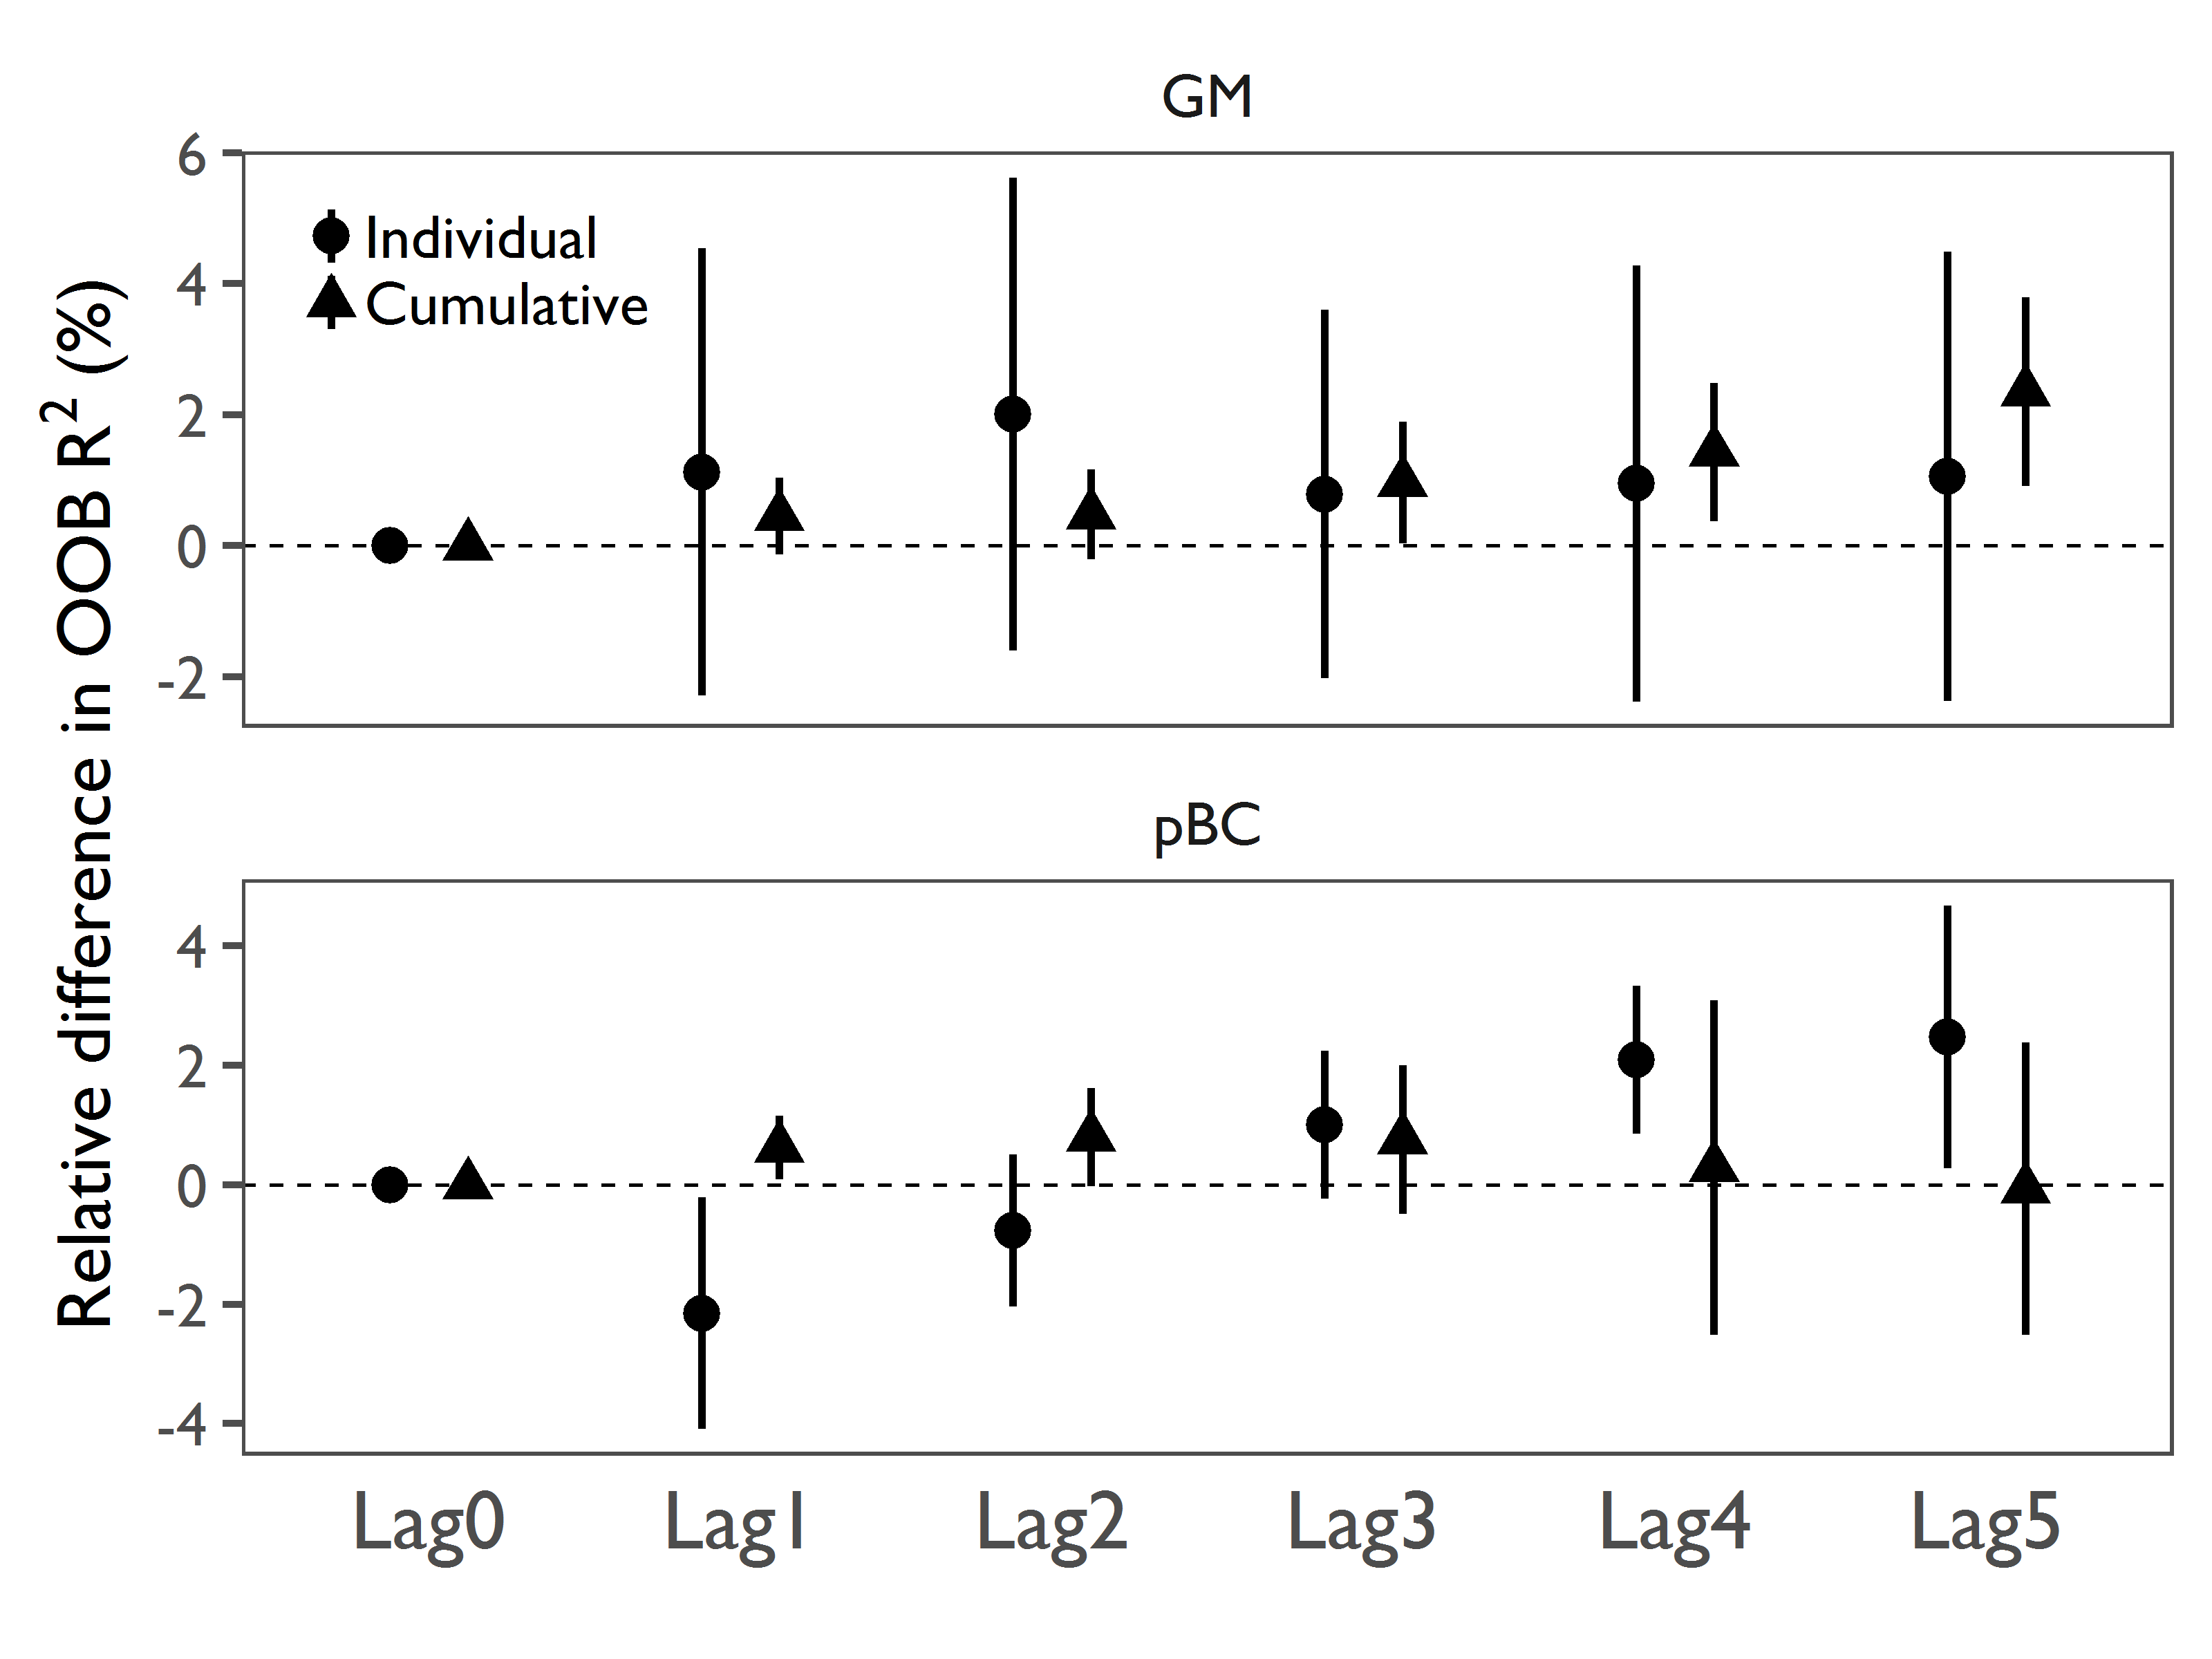
\includegraphics[width=1\textwidth]{chapter4/F03}
\caption{ Difference in local biodiversity measures between sites with varying sequences of land cover relative to sites without any past land-cover change (dotted line) in the period 1992 to biodiversity sampling start. Separate models were fitted for each biodiversity measure and land cover at the time of biodiversity sampling as indicated by colour and abbreviation, namely forest (F, \textbf{a}), shrubland (Sh, \textbf{b}), grassland (G, \textbf{c}), sparse vegetation (SV, \textbf{d}), agriculture (A, \textbf{e}) and urban (U, \textbf{f}). Abbreviations on the x-axis show the difference in local biodiversity (SR = Species richness, LA = Total abundance, PIE = Species assemblage evenness). Number of sites contributing to each fitted land-cover sequence are indicated. The error bars show the predicted standard error and stars (*) indicate whether the difference is statistically significant (p < 0.05).}
\label{F04_03}
\end{figure}
% -------------------------------------------- %

Local biodiversity varied globally with land cover in the year 2015 as estimated from spatial projections (Figure \ref{F04_04}\textbf{a}). Predicted biodiversity estimates across grid cells had a range from 41\% to 0\% fewer species, 10\% to 13.3\% fewer individuals and 30.3\% to 46.1\% less even assemblages. Globally projected differences in species richness had considerable uncertainty ranging between $\pm$ 0.1\% and $\pm$ 29\% MAE in the most extreme cases (grid cells with over 5.5\% MAE occurred in less than 1\% of all land grid cells). Informed by past land-cover sequences (Figure \ref{F04_03}), we found the predicted number of species to be up to 17.1\% lower or 20.1\% higher than those predicted estimates that do not take sequences of past land cover into account (Appendix Figure \ref{SI04_03}). This is especially the case for locations in the Amazon and Gran Chaco (Figure \ref{F04_01}\textbf{b}), where after \textendash\ accounting for land-cover change between 2000 and 2015 \textendash\ high losses of species are expected (Figure \ref{F04_04}\textbf{b}). Projections were created using human population density as covariate and we found that a greater human population density increased species richness in sparse vegetation, agriculture and urban covered sites relative to forest covered grid cells, while total abundance increased with human population density across all land-cover categories relative to forest covered grid cells (Appendix Figure \ref{SI04_04}).

% ---------------- Figure 4 --------------------- %
\begin{figure}[!h]
\centering
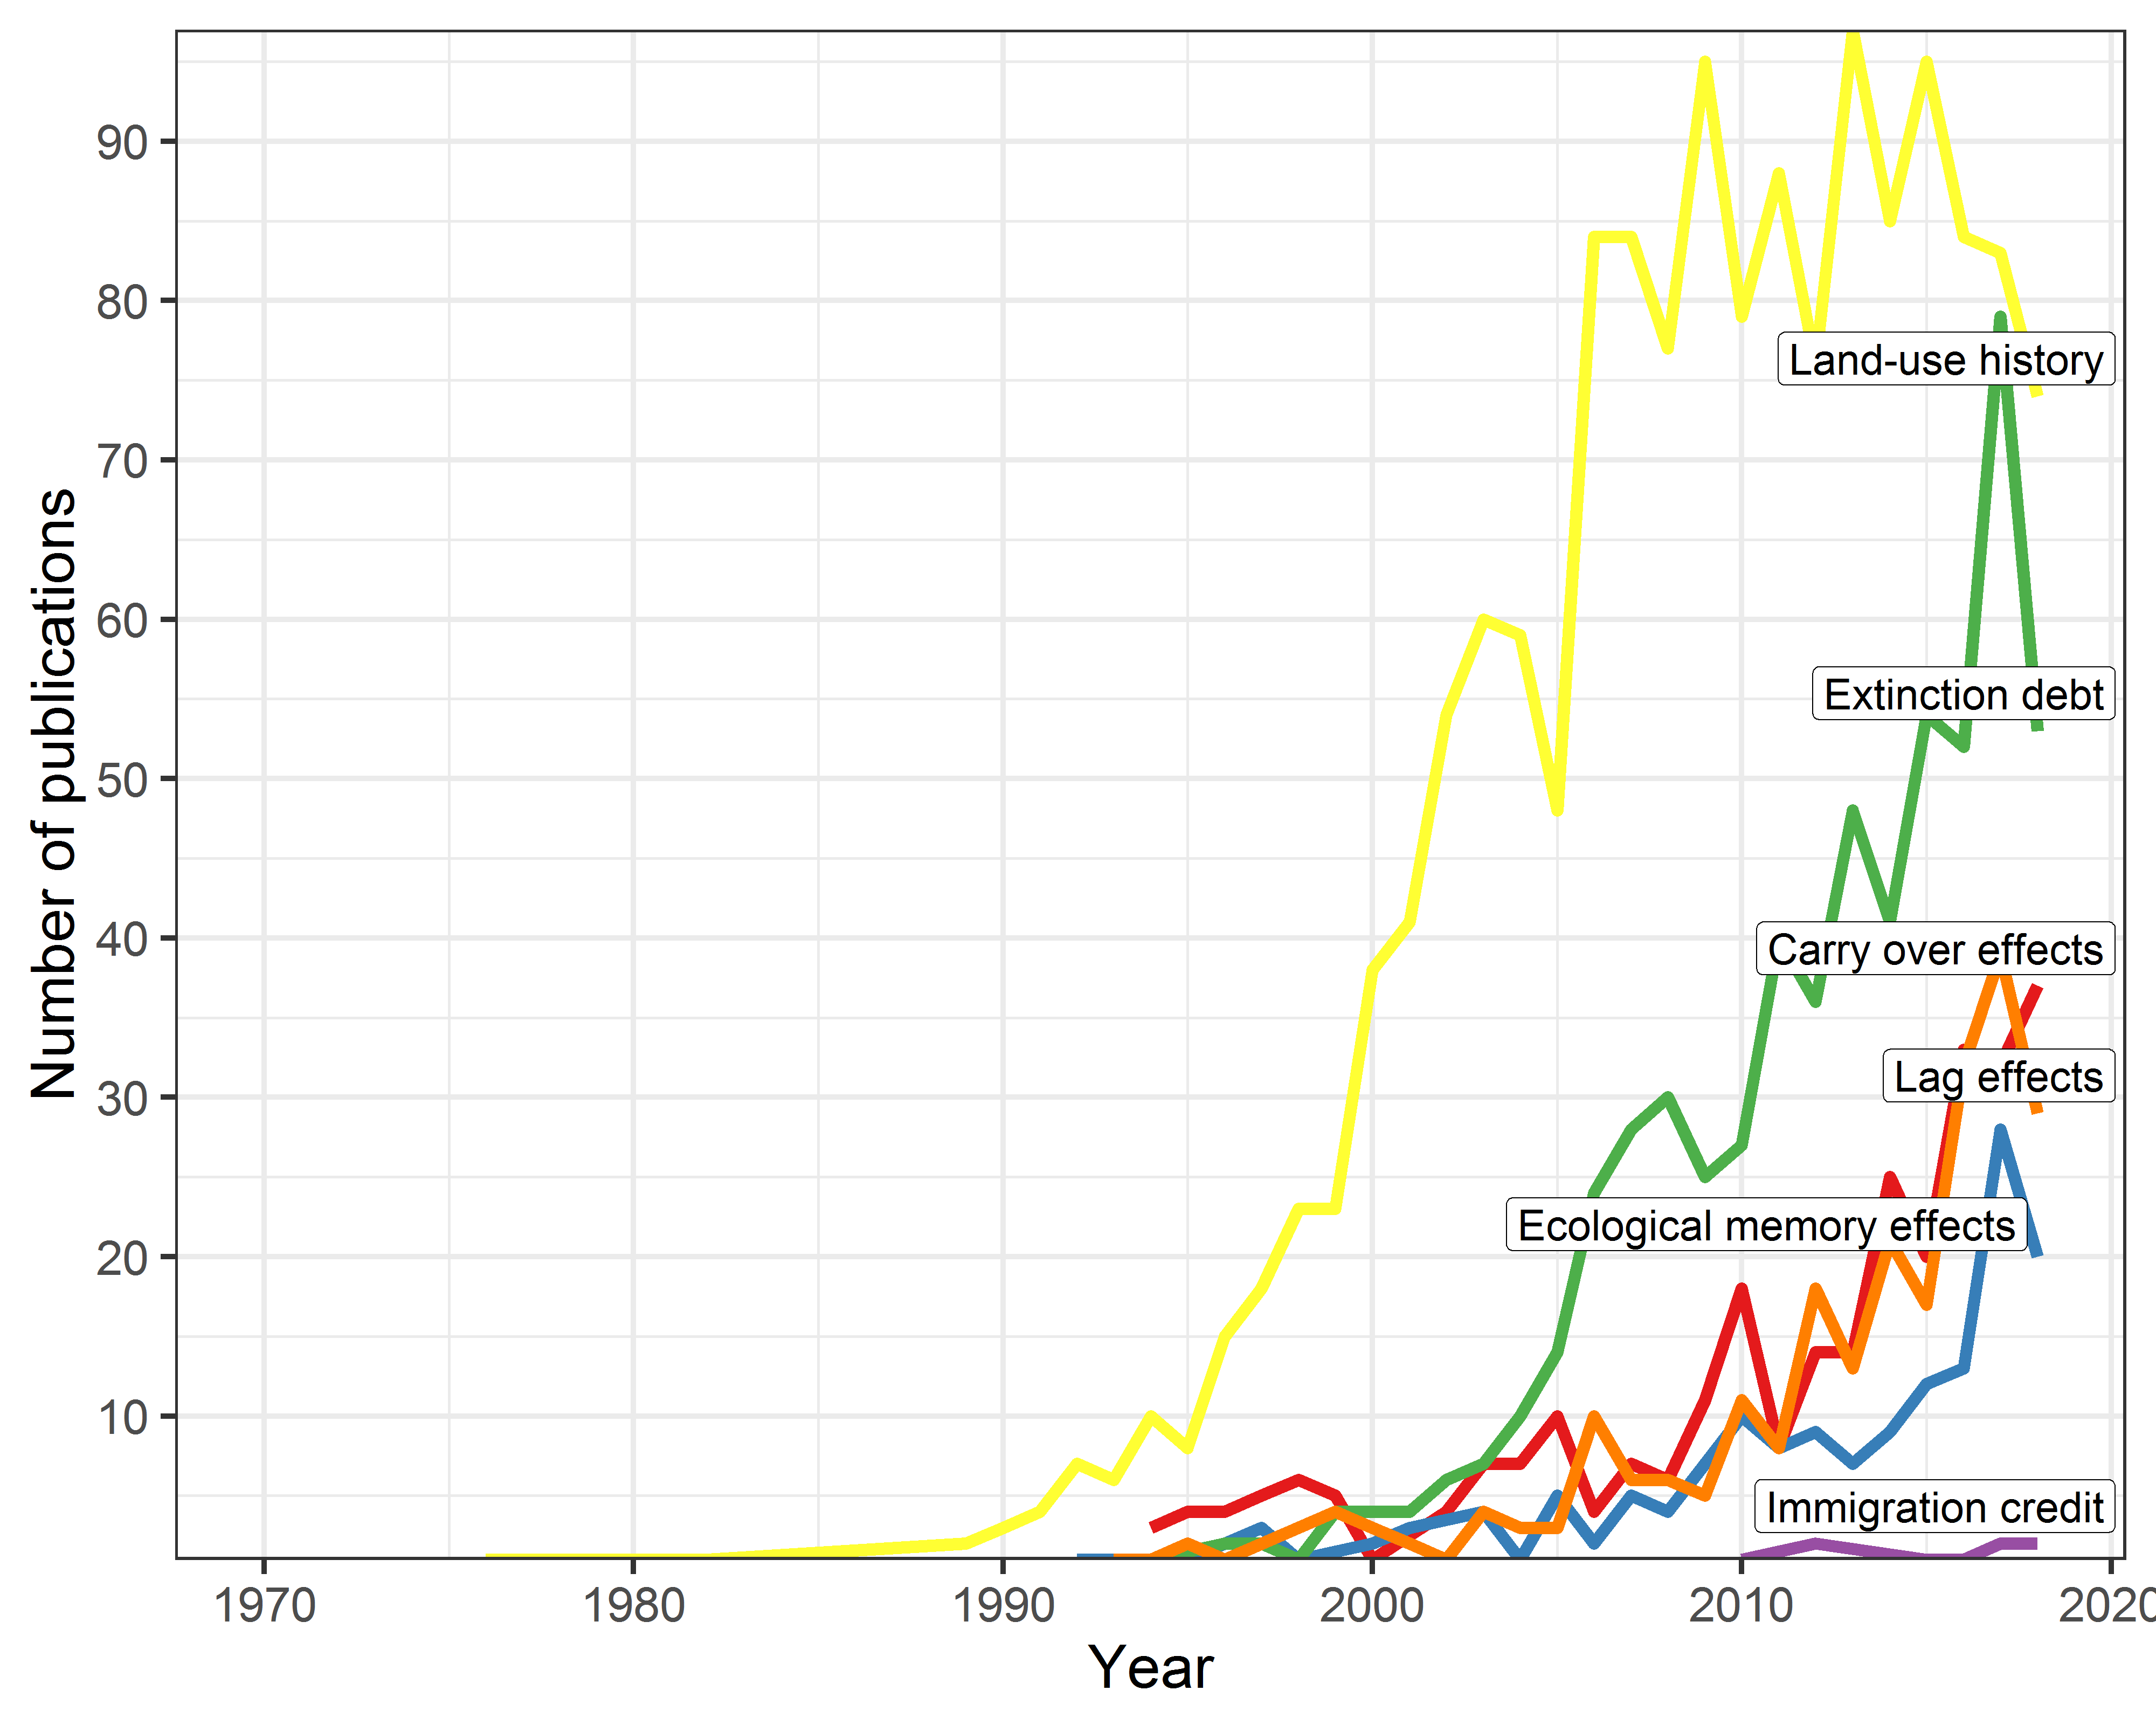
\includegraphics[width=1\textwidth]{chapter4/F04}
\caption{ (\textbf{a}) Global projection of the difference in local species richness with land cover \textendash\ relative to a forest site with zero human population \textendash\ and informed by land-cover sequences in the past. Projected biodiversity estimates are visualized relative to their uncertainty (normalized mean absolute error (MAE) from the predicted difference), where values of higher uncertainty are visually suppressed in hue. Most extreme values (lowest 1\% and highest 1\% percentile) were excluded from the visualization and are displayed as inland white colour. (\textbf{b}) shows examples (as in Figure \ref{F04_01}) how projections of local species richness loss differ because of prediction uncertainties and land-cover sequences. Map is displayed in a global equal-area Mollweide projection and aggregated to \textasciitilde 3km\textsuperscript{2} resolution for this visualization. Predicted difference and uncertainty (unweighted) are in Appendix Figure \ref{SI04_03} individually. }
\label{F04_04}
\end{figure}
% -------------------------------------------- %

Land cover changes continue to influence predicted biodiversity estimates at the national scale. On average 4.04\% $\pm$ 3.73 SD of land across all countries had a land-cover change relative to their total land area in the period from 2000 to 2015. Singapore with 31.7\%, Malawi with 17.7\% and Paraguay with 16.4\% had the highest proportion of land with a land-cover change in the period 2000 to 2015 (Appendix Figure \ref{SI04_05}). Although there were no significant differences in the proportion of land with a land-cover change among countries ($F_{2,201}$=0.477, p=0.621, Appendix Figure \ref{SI04_05}), considering past land-cover change affected biodiversity more in tropical, lower-income countries (Figure \ref{F04_05}, Appendix Figure \ref{SI04_06}-\ref{SI04_07}). The area-weighted difference in projected national biodiversity estimates \textendash\ relative to a projection that did not account for land-cover sequences \textendash\ was significantly lower in low income countries for species richness ($F_{2,200}$=9.131, p<0.001, Figure \ref{F04_05}), total abundance ($F_{2,198}$=13.48, p<0.001, Figure \ref{SI04_06}) and evenness ($F_{2,198}$=6.644, p<0.01, Appendix Figure \ref{SI04_07}).

% ---------------- Figure 5 --------------------- %
\begin{figure}[hb]
\centering
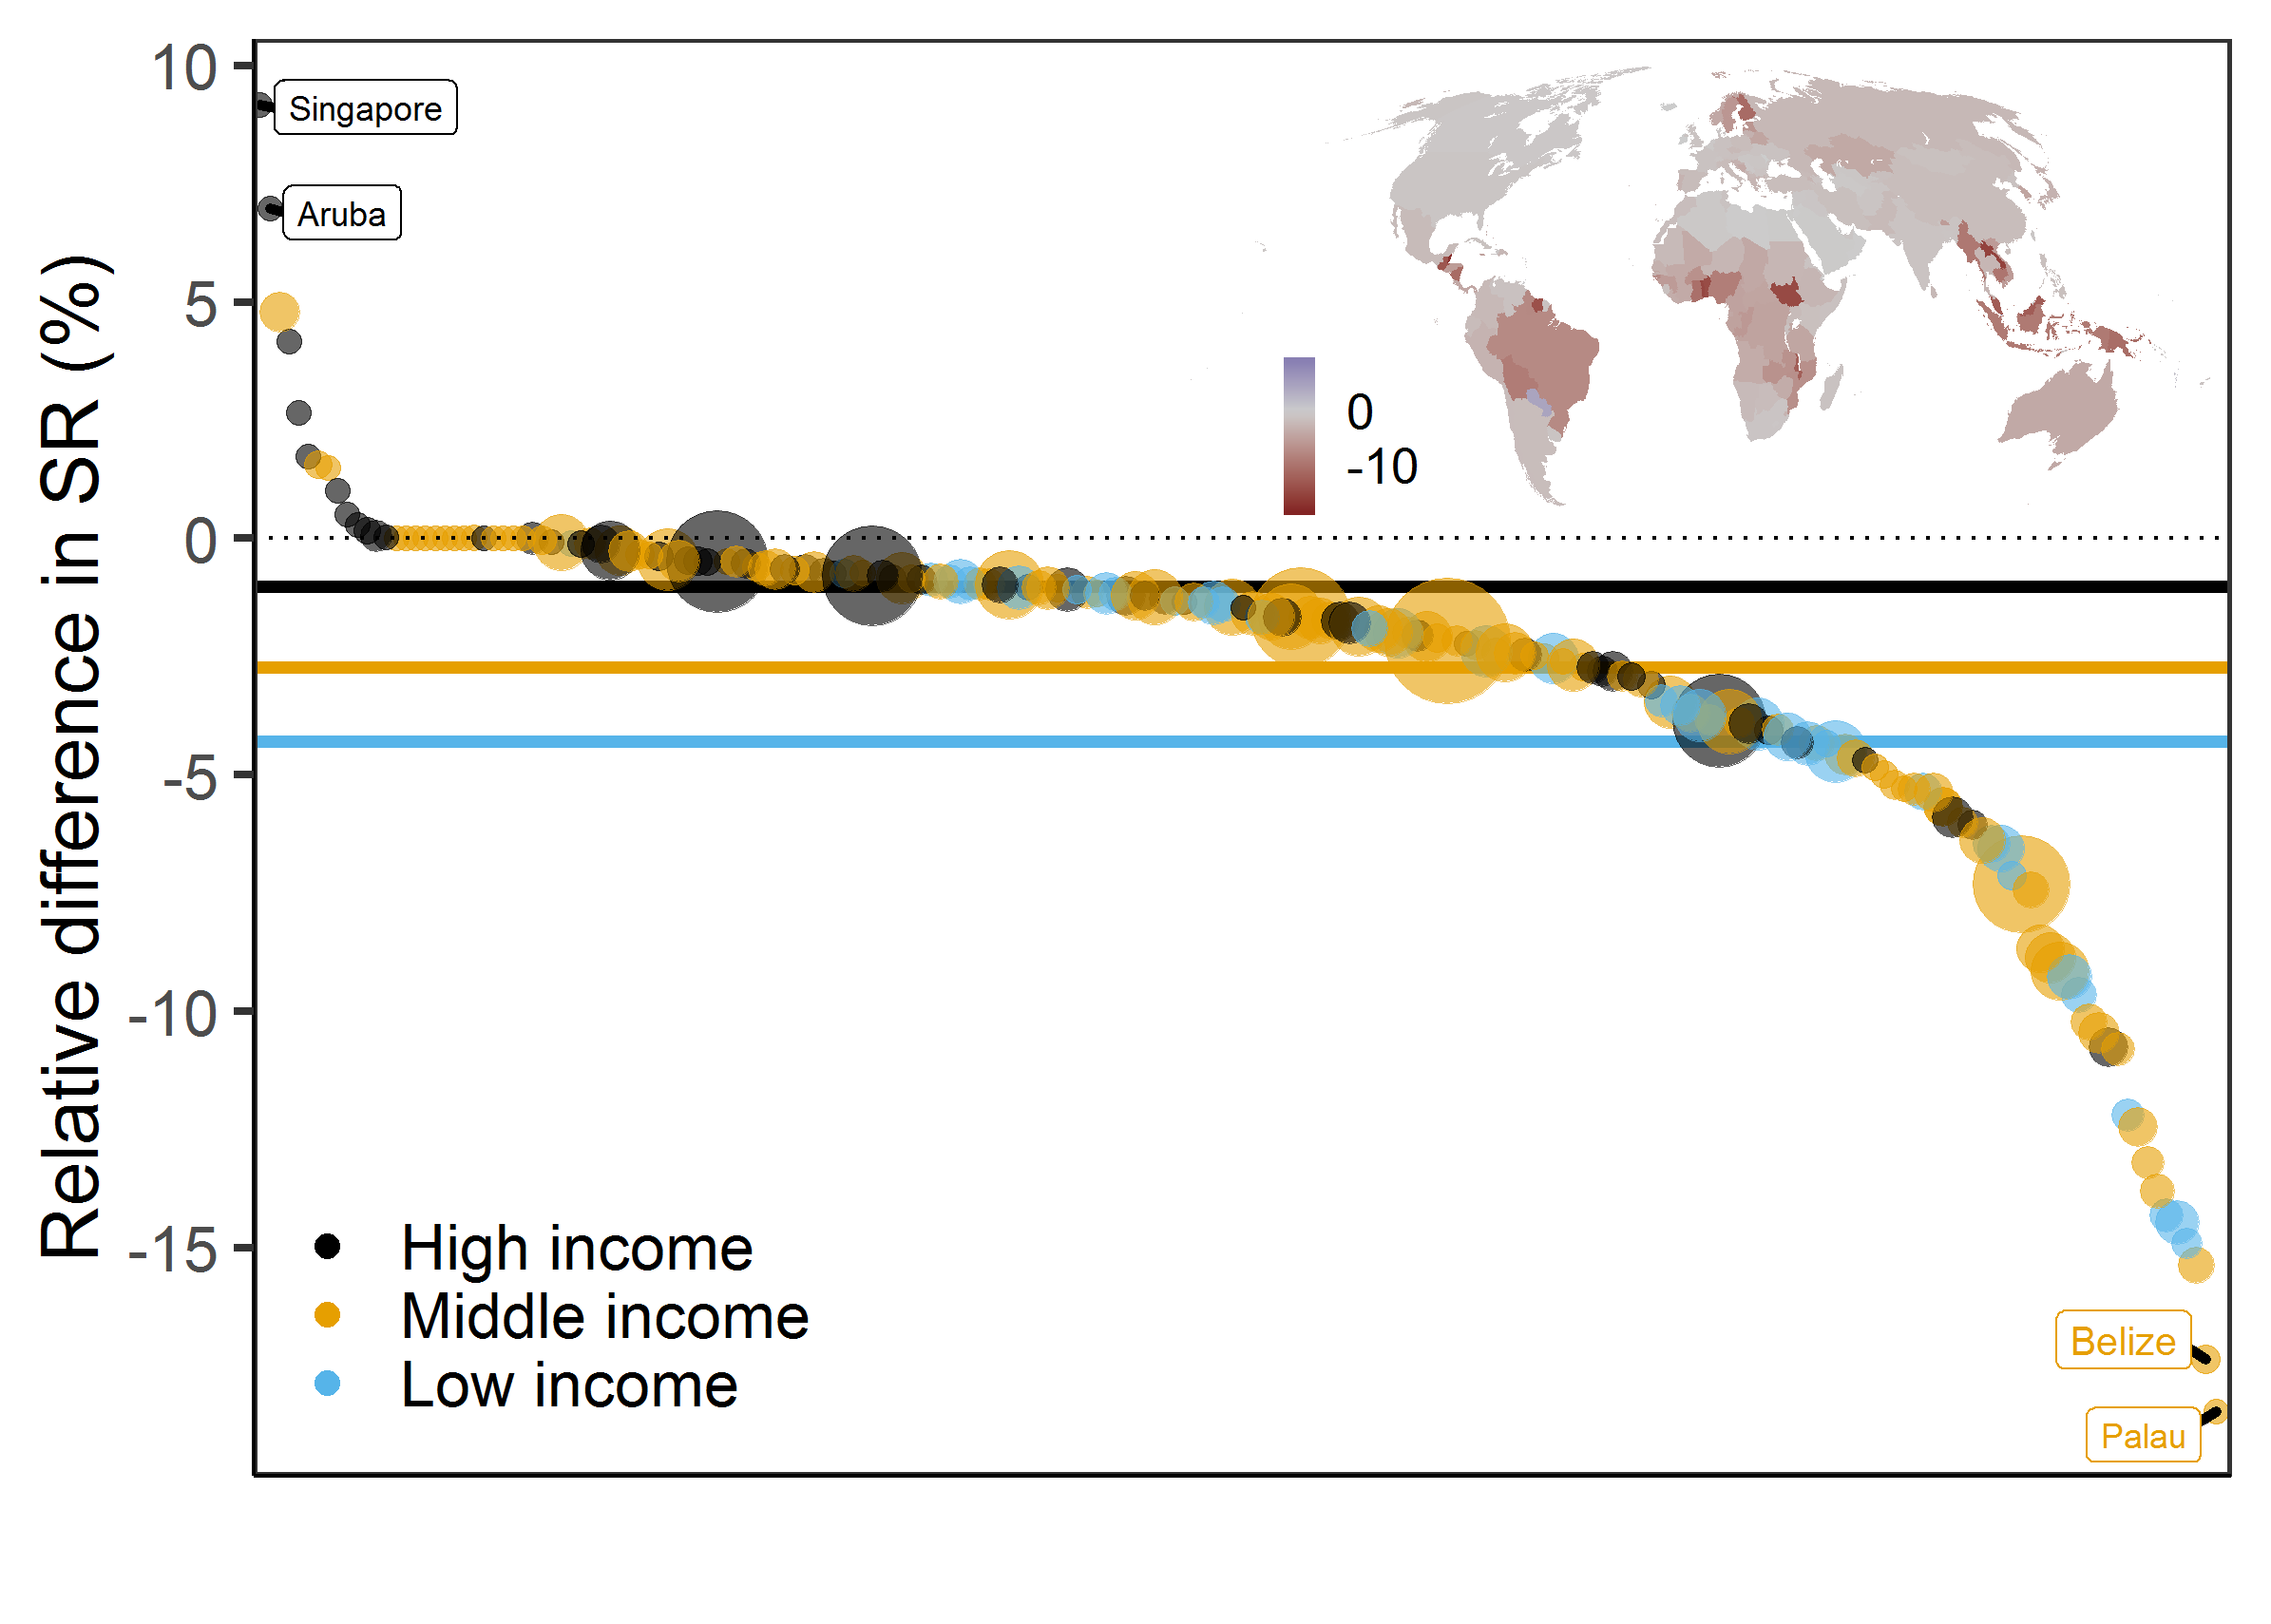
\includegraphics[width=1\textwidth]{chapter4/F05}
\caption{ Area-weighted relative difference \textendash\ compared to a projection where past land-cover sequences were not considered \textendash\ in mean national species richness (SR) from 2000 to 2015. Points represent the country-wide average in SR (area-weighted) with the size of the points scaled with land area (small to large). Colours indicate whether countries are considered high (black), middle (orange) or low (blue) income. Outlier countries and overall averages per income group (horizontal lines) are indicated. Inset map shows the relative difference in SR from low (red) to high (blue) per country. Plots for total abundance and assemblage evenness are broadly comparable (Appendix Figure \ref{SI04_06} - \ref{SI04_07}). }
\label{F04_05}
\end{figure}
% -------------------------------------------- %

\section{Discussion}
\label{C04_04}

Biodiversity is expected to differ with attributes of past land-cover change \citep{Watson2014}. We found local biodiversity at sites with a past land-cover change to be on average lower than at sites without any land-cover change in the period 1992 to biodiversity sampling start. Local biodiversity recovered to levels comparable to sites without land-cover change after more than ten years had passed (Figure \ref{F04_02}). These results are in line with a previous study on the same biodiversity dataset that found abrupt land changes to consistently reduce local biodiversity (Chapter \ref{C03} in this thesis). We furthermore found that the impacts of land-cover change on biodiversity varied with different sequences of past land cover (Figure \ref{F04_03}) and that these impacts affect global (Figure \ref{F04_04}) and national (Figure \ref{F04_05}) biodiversity projections. We discuss how our results relate to those of previous studies and make recommendations how to incorporate lasting influences of past land-cover change into biodiversity projections.

\subsection{The influence of land-cover sequences on biodiversity}
\label{C04_0401}

Depending on the sequence of land cover, local biodiversity measures were considerably altered after a land-cover change. Forest covered sites, that were previously covered by agriculture, had about the same number of species and individuals as forest covered sites without a land-cover change in the period 1992 to biodiversity sampling start (Figure \ref{F04_03}\textbf{a}), which contrasts with findings of previous studies investigating the impacts of an agriculture to forest transition on local biodiversity \citep{Bellemare2002,Hermy2007,Dyer2010}. It could be that many of the reference forest-covered sites had an agricultural history long before 1992 \textendash\ which we were unable to quantify using the ESA LC product \textendash\ potentially weakening the impacts of land-cover change as local biodiversity has already been noticably altered before the start of satellite-based earth observation \citep{Ellis2010,McMichael2017}. A previous meta-analysis has shown that forests, which were previously covered by shrublands had on average lower species richness \citep{Bremer2010} and we found similar results with previously shrub covered sites, having on average 11\% fewer species and 14\% fewer individuals (Figure \ref{F04_03}\textbf{a}). In contrast, previously forest covered shrubland sites had on average 11\% more species and 26\% more individuals than a shrubland site without a past land-cover change (Figure \ref{F04_03}\textbf{b}). Likely these sites still support a high number of species typical at low vegetation height and structural complexity \citep{Chazdon2016}. 

In more anthropogenically altered land cover, a past land-cover change caused varying “biotic lag” effects (Figure \ref{F04_03}\textbf{e}-\textbf{f}). Urban sites with a past land-cover change had a higher number of species and individuals than sites without land-cover change (Figure \ref{F04_03}\textbf{f}). It could be that local biodiversity in these sites is inflated because of pending extinction debts and thus these sites likely have further extinctions of (native) species in the future \citep{Tilman1994,Kuussaari2009,Hylander2013}. This is supported by a previous global synthesis that found preceding land cover together with city age to be one of the best predictors of (native) bird and plant occurrence in urban areas \citep{Aronson2014}. However, similar effects could not be observed for agricultural sites previously covered by forest or shrubland, where the number of species and individuals was on average lower compared to an agricultural site without a past land-cover change (Figure \ref{F04_03}\textbf{e}). One possible explanation could be that this pattern is mostly driven by (pollinating) invertebrates, which compose 64.8\% of all previously forest or shrub covered agricultural sites in our dataset. Pollinating invertebrates have previously been shown to have higher numbers of species and individuals in agricultural land compared to forests \citep{Winfree2009}. It should be mentioned that many of our findings could be rather imprecise given the low number of sites with a past land-cover change (Appendix Figure \ref{SI04_02}), which prevented us from robustly assessing the impact of land-cover sequences across taxonomic or functional groups \citep{Jung2018} or in interactions with other attributes of land-cover change such as time passed (Figure \ref{F04_02}). Nevertheless, this is to our knowledge the first comprehensive and comparative assessment of the impacts of past land-cover sequences on local biodiversity measures.

The consideration of past land-cover change can also affect global and national biodiversity projections (Figure \ref{F04_04} \& \ref{F04_05}). Notably only 4.04\% of the terrestrial land surface globally had a land-cover change in the period 1992 to 2015 occurring predominantly in the global south (Figure \ref{F04_01}). Previous studies that analysed the spatial distribution and drivers of land-cover change \citep{Curtis2018,Nowosad2018} found the expansion of agriculture and pasture to be the most likely cause of land-cover change in those areas \citep{Phalan2013}, which are often globally irreplaceable for biodiversity \citep{Brooks2002,Laurance2014b,Pimm2014}. Comparing national biodiversity projections with and without a consideration of past land-cover change, we find that a consideration of land-cover sequences led to even lower predicted national biodiversity estimates in most, but especially so in tropical and low-income countries (Figure \ref{F04_05}, Appendix Figure \ref{SI04_06}-\ref{SI04_07}). In those countries anthropogenically caused land-cover change is commonly linked to attempts to close yield-gaps in agricultural production \citep{Mueller2012a} or increase the output of export commodities \citep{Byerlee2014,Meyfroidt2018}. Our results indicated that not accounting for lagged effects of past land-cover change can cause an over- and/or underestimation of biodiversity change in global projections.

\subsection{Model and land cover data uncertainties in biodiversity projections}
\label{C04_0402}

There are several factors that need to be considered when our results are compared to those of previous studies \citep{Newbold2015}. The PREDICTS database was set up to compare biodiversity measures between sites of varying land-use and land-use intensity as derived from study descriptions \citep{Newbold2015,Hudson2016}, while this study used remotely-sensed estimates of land cover. Land use and land cover are intertwined in a land system \citep{Lambin2006,Turner2007}, however not all differences between two PREDICTS sites can likely be explained by land cover (and human population density, Appendix Figure \ref{SI04_03}) alone. Differences in impacts can occur because of inaccuracies in characterizing land cover \citep{ESA2017}, scale mismatches \citep{Estes2018} or local factors that mediate biodiversity responses to differences in land cover \citep{Jung2016}. Furthermore because of sampling size limitations, we were not able to incorporate other attributes of land-cover change that could be important in determining differences in local biodiversity measures \citep{Watson2014}, such as the frequency \citep{Watson2014,Griffiths2015} or magnitude of land-cover change (Chapter \ref{C03} in this thesis). Future studies should attempt to incorporate interactions between attributes of land-cover change into biodiversity projections, pending greater biodiversity and land-cover data availability.

Remotely characterizing land-use and/or land-cover at global extents is challenging \citep{VERBURG2011,Kuemmerle2013}. In this study we used time series (period 1992-2015) of remotely-sensed land cover instead of the modelled estimates (1500-2100) of land use and land cover \citep{Hurtt2011,KleinGoldewijk2016} used by previous studies \citep{Newbold2015,Newbold2016b,DePalma2017}. Most of the terrestrial land surface has been altered by humans long before the availability of Earth observation data \citep{Ellis2010} and modelled estimates of land-use change are often the only available data at global scales. However, these estimates are only available at coarse spatial resolution (\textasciitilde 10 km\textsuperscript{2} at the equator) and are dependent on model assumptions and accompanied uncertainties \citep{Gaillard2010,KleinGoldewijk2013}, with previous independent validations having shown that they can misrepresent pre-industrial land use substantially \citep{Kaplan2017}. Remotely-sensed land-cover products, despite classification errors and thematic differences that can affect subsequent analyses \citep{Sexton2015,Estes2018}, remain some of the best directly measured estimates of global land cover, but not land use. Promising case studies have quantified proxies of land use for agricultural \citep{Estel2015}, pasture \citep{Rufin2015} or forest use intensity \citep{Pflugmacher2012} from time series of remotely-sensed data at the regional scale. We suggest that in order to improve future biodiversity models and projections, new time series of remotely-sensed proxies of land use need to be developed at the global scale. 

\subsection{Conclusion}
\label{C04_0403}

This study investigated the impacts of past land-cover change \textendash\ differentiated by attributes such as time passed or the sequence of land cover \textendash\ on local biodiversity. We found local biodiversity to be significantly reduced shortly after a land-cover change but being able to recover with longer time passed (Figure \ref{F04_02}). Depending on the sequence of past land cover, local biodiversity either increased or decreased compared to sites without a land-cover change (Figure \ref{F04_03}). If those lasting influences of past land-cover change are ignored in global and national biodiversity projections, we find that those projections can considerably misrepresent projected biodiversity change, especially so in tropical and low-income countries (Figure \ref{F04_04} - \ref{F04_05}). There are several ways to improve biodiversity projections beyond of what has been presented in this study. We emphasize the need to consider interactions between attributes of land-cover change such as between the time passed (Figure \ref{F04_02}) and land-cover sequences (Figure \ref{F04_03}), which might affect the estimated impacts on biodiversity given evidence from previous studies \citep{Chazdon2003,Martin2013}. The impacts of land-cover change could furthermore be estimated using before and after biodiversity measures \citep{DePalma2018} and time series of land cover could be useful to identify sites for resurveying local biodiversity (see figure \ref{F06_01} in discussion) or to establish links with time series of biodiversity measures \citep{Dornelas2018}. Overall, our study highlights the usefulness of remotely-sensed time series of land cover for biodiversity projections and models, particularly in quantifying lasting impacts of past land cover change.

\clearpage
%\bibliography{content/04Chapter}

%\appendix
%\begingroup
%  % SI - Figure 1 Missing data
\begin{figure}[h]
\centering
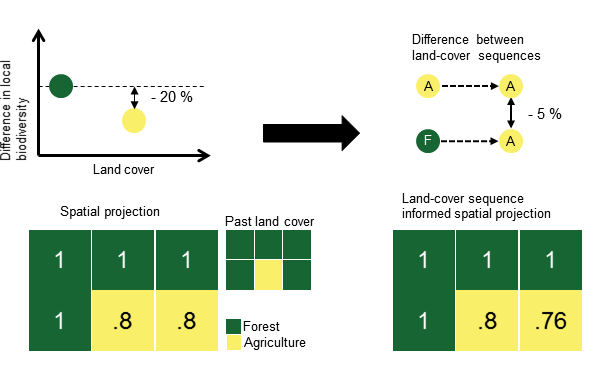
\includegraphics[width=1\textwidth]{chapter3/SI01}
\caption{ Average temporal distribution of Landsat data and an example times series of Landsat data. (\textbf{a}) Distribution of available Enhanced Vegetation Index (EVI) data in years covered by the Landsat missions. Points show the average monthly EVI data availability per year (0 to 12 months of data) across time series and PREDICTS sites grouped by 15\textdegree latitude bins. The size of points indicates the mean data availability (0 to 100\% with 100\% having 12 months of available data in a given year), while the colour shows the number of PREDICTS sites contributing to the mean (as PREDICTS sites were sampled in varying years). (\textbf{b}) Example time series for one PREDICTS site with a high proportion of missing data before 1999. In all analyses such time series were truncated to the period from 1999 onwards (indicated by the dashed line).}
\label{SI03_01}
\end{figure}

% SI - Figure 2 Binning
\begin{figure}[h]
\centering
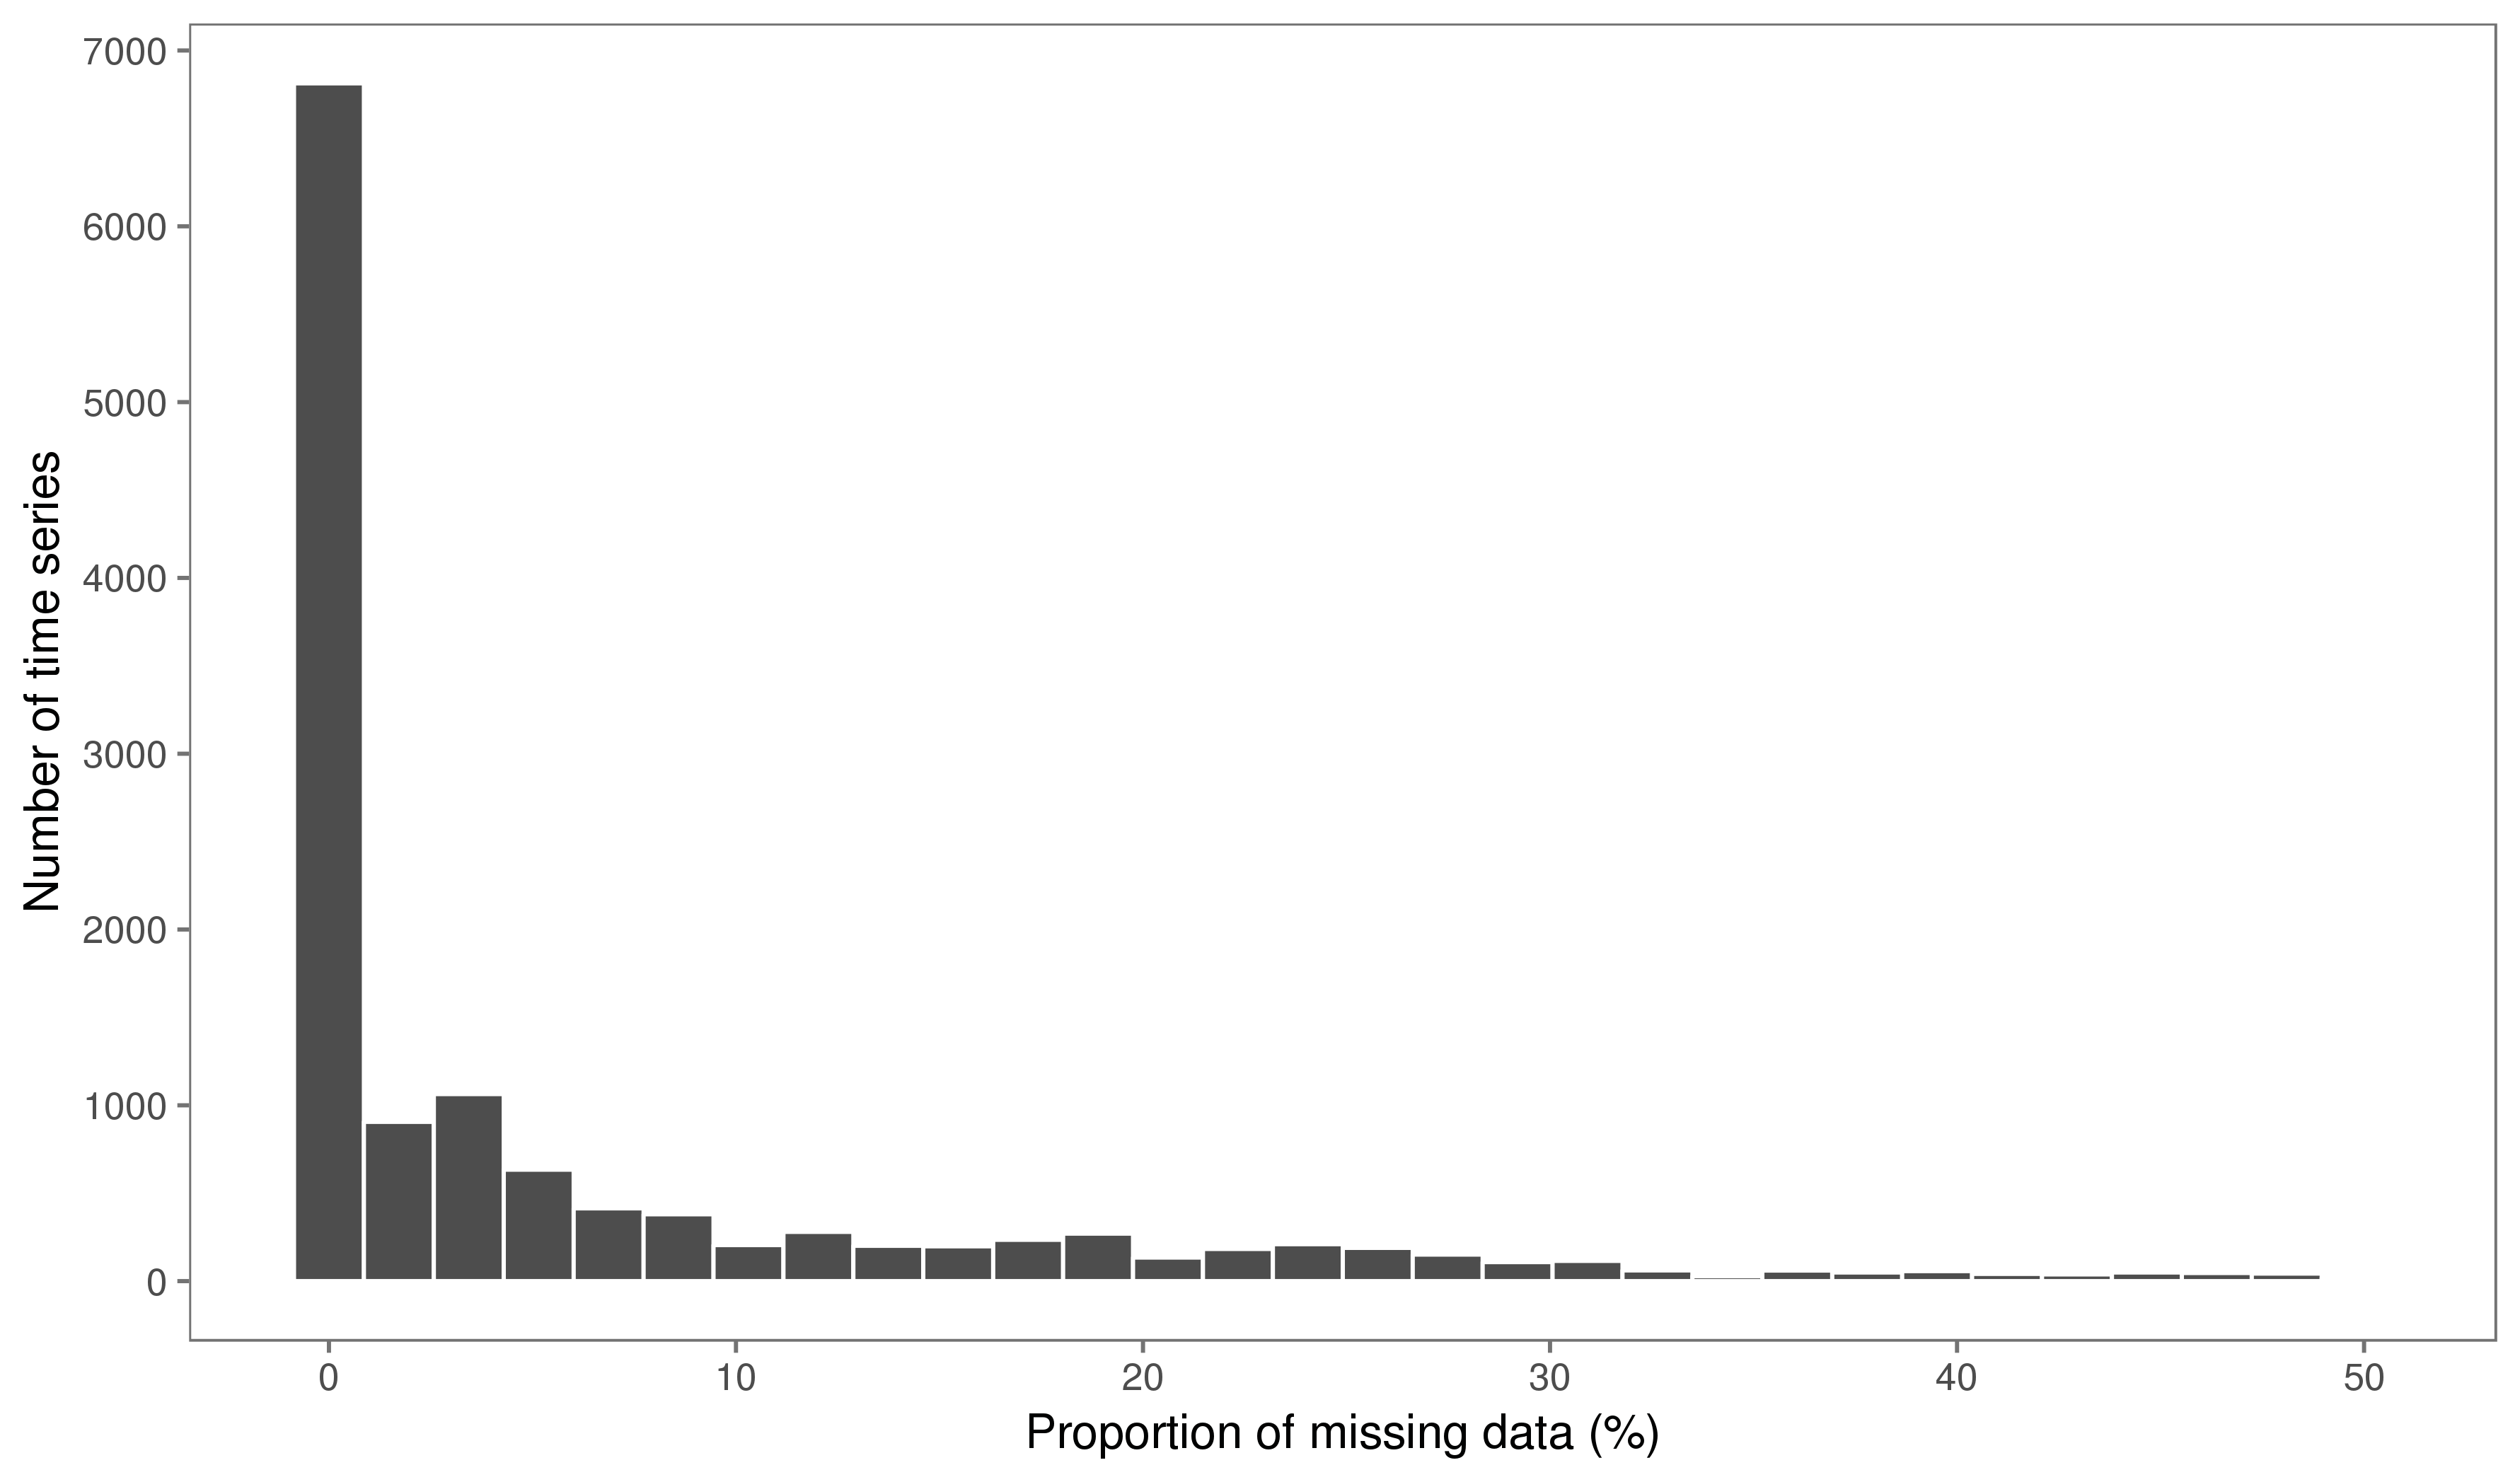
\includegraphics[width=1\textwidth]{chapter3/SI02}
\caption{ Number of sites with abrupt land change per attribute. Number of sites (black line) per attribute of abrupt land change with (\textbf{a}) the relative shift in magnitude, (\textbf{b}) the shift in trend as difference in annual EVI trend, and (\textbf{c}) the time passed between abrupt land change and biodiversity sampling. Background colours in (\textbf{a}) and (\textbf{b}) indicate the binning into six groups for shifts in magnitude (> 50\%, > 25\% to $\leq$ 50\%, and $\leq$ 25\% EVI loss [$---$ to $-$] or gain [$+++$ to $+$]), and in trend (0.01, 0.05, and > 0.05 annual negative [$---$ to $-$] to positive [$+++$ to $+$] EVI trend differences). Gray lines in (\textbf{c}) delineate bins of time passed ($\leq$ 5 years, > 5 and $\leq$ 10 years, and >10 years). Colours as in Figure \ref{F03_02}.}
\label{SI03_02}
\end{figure}

% SI Table 1------ %
% From here https://www.tablesgenerator.com/
\begin{table}[]
\centering
\caption{Number of PREDICTS sites and studies with an abrupt land change. Shown as either a change in magnitude (columns) and/or change in trend (trend). Symbols as in Figure \ref{F03_02}. }
\label{SIT03_01}
\begin{tabular}{@{}lllllllllll@{}}
                                          &                                           & \multicolumn{7}{c}{\textbf{Shift in magnitude}}                                                                                                                                                                    &                               &                             \\
                                          &                                           & \textbf{- - -}             & \textbf{- -}                & \textbf{-}                   & \textbf{0}                    & \textbf{+}                   & \textbf{+ +}                & \textbf{+ + +}              & \textbf{Total sites}          & \textbf{Studies}            \\ \cmidrule(l){3-11} 
                                          & \multicolumn{1}{l|}{- - -}                & 2                          & 8                           & 192                          & NA                            & 73                           & 26                          & 22                          & \cellcolor[HTML]{EFEFEF}323   & \cellcolor[HTML]{C0C0C0}57  \\
                                          & \multicolumn{1}{l|}{- -}                  & 7                          & 281                         & 642                          & NA                            & 497                          & 158                         & 53                          & \cellcolor[HTML]{EFEFEF}1638  & \cellcolor[HTML]{C0C0C0}175 \\
                                          & \multicolumn{1}{l|}{-}                    & 7                          & 88                          & 256                          & NA                            & 231                          & 154                         & 53                          & \cellcolor[HTML]{EFEFEF}789   & \cellcolor[HTML]{C0C0C0}184 \\
                                          & \multicolumn{1}{l|}{0}                    & NA                         & NA                          & NA                           & 10102                         & NA                           & NA                          & NA                          & \cellcolor[HTML]{EFEFEF}10102 & \cellcolor[HTML]{C0C0C0}358 \\
                                          & \multicolumn{1}{l|}{+}                    & 9                          & 102                         & 399                          & NA                            & 410                          & 205                         & 49                          & \cellcolor[HTML]{EFEFEF}1174  & \cellcolor[HTML]{C0C0C0}237 \\
                                          & \multicolumn{1}{l|}{\textbf{+ +}}         & 47                         & 172                         & 342                          & NA                            & 465                          & 254                         & 86                          & \cellcolor[HTML]{EFEFEF}1366  & \cellcolor[HTML]{C0C0C0}224 \\
\multirow{-7}{*}{\textbf{\rotatebox{90}{Shift in trend}}} & \multicolumn{1}{l|}{\textbf{+ + +}}       & 12                         & 137                         & 47                           & NA                            & 34                           & 12                          & 31                          & \cellcolor[HTML]{EFEFEF}273   & \cellcolor[HTML]{C0C0C0}56  \\
                                          & \multicolumn{1}{l|}{\textbf{Total sites}} & \cellcolor[HTML]{EFEFEF}84 & \cellcolor[HTML]{EFEFEF}788 & \cellcolor[HTML]{EFEFEF}1878 & \cellcolor[HTML]{EFEFEF}10102 & \cellcolor[HTML]{EFEFEF}1710 & \cellcolor[HTML]{EFEFEF}809 & \cellcolor[HTML]{EFEFEF}294 &                               &                             \\
                                          & \multicolumn{1}{c|}{\textbf{Studies}}     & \cellcolor[HTML]{C0C0C0}34 & \cellcolor[HTML]{C0C0C0}135 & \cellcolor[HTML]{C0C0C0}246  & \cellcolor[HTML]{C0C0C0}358   & \cellcolor[HTML]{C0C0C0}263  & \cellcolor[HTML]{C0C0C0}171 & \cellcolor[HTML]{C0C0C0}83  &                               &                            
\end{tabular}
\end{table}
% ------ %

% SI - Figure 3 Cross-correlations
\begin{figure}[h]
\centering
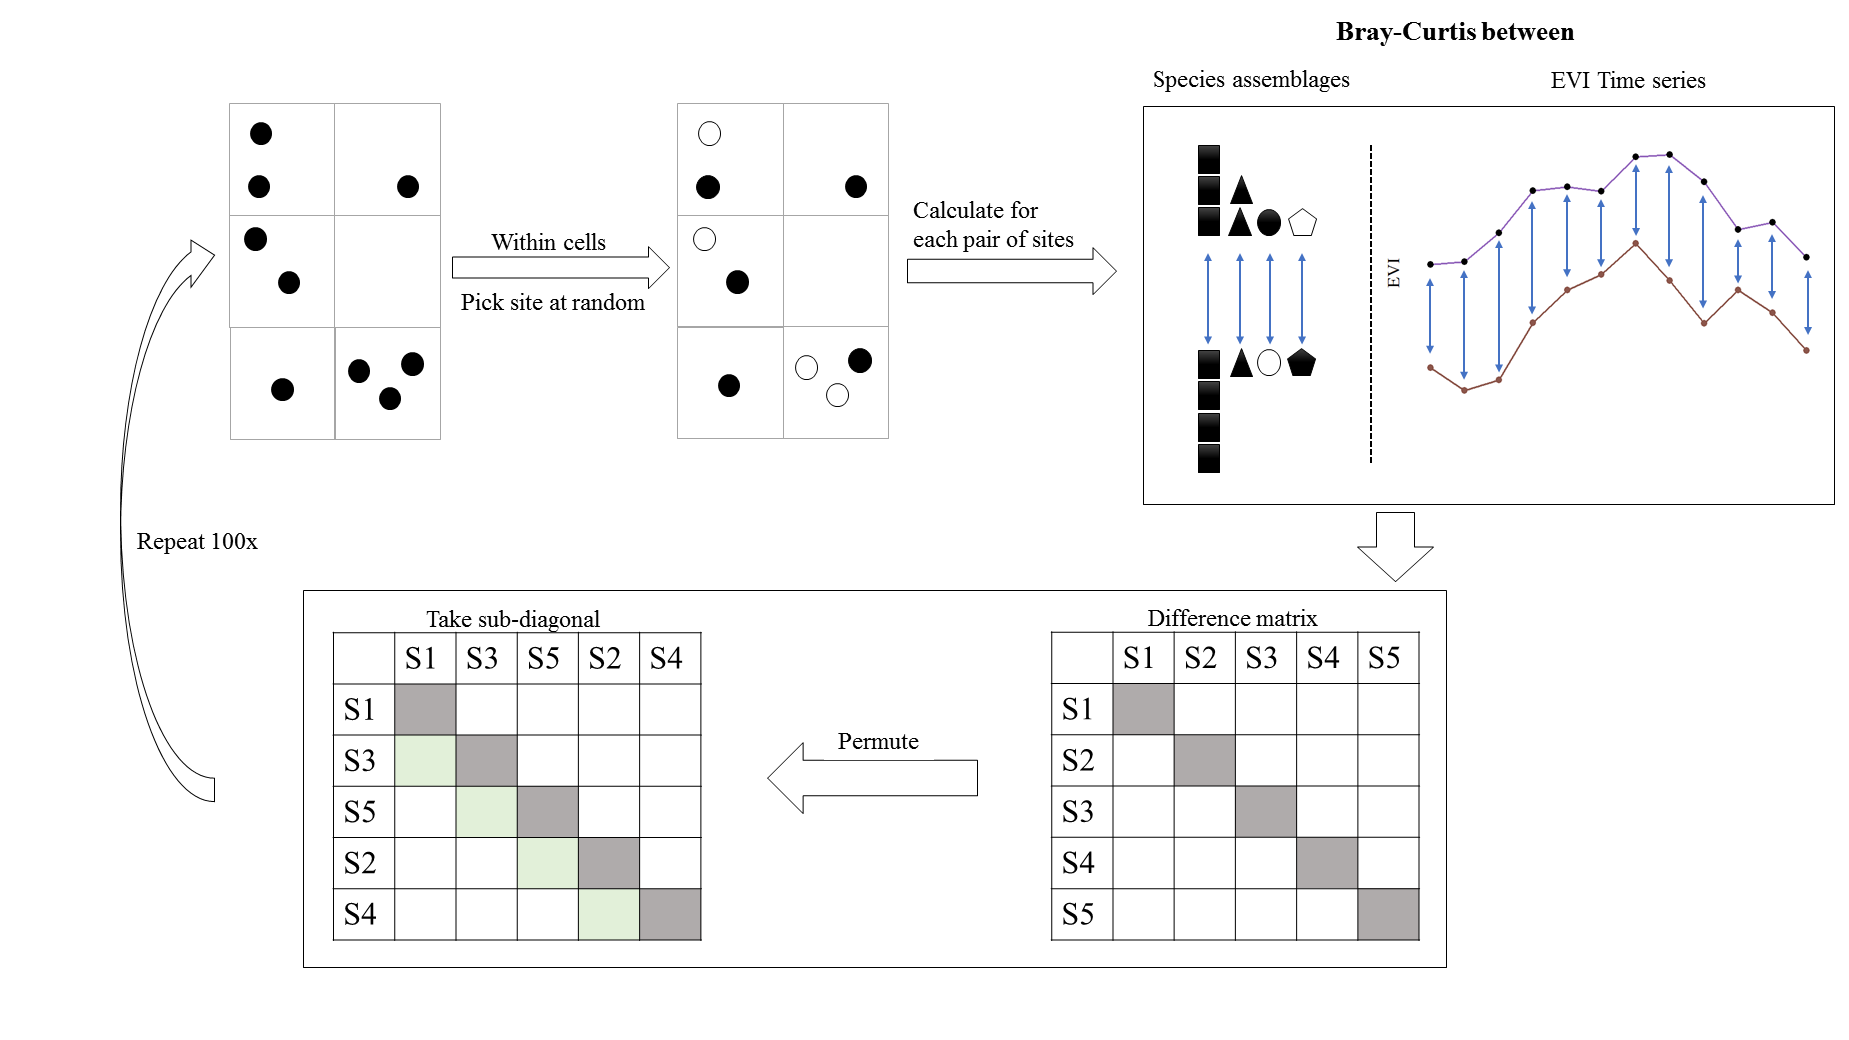
\includegraphics[width=1\textwidth]{chapter3/SI03}
\caption{ Correlations between attributes of abrupt land change. Showing shifts in magnitude, trend and time passed (see Methods). The lower facets show a point density plot, the upper facets the Pearson correlation coefficient between pairs of attributes and the diagonal a density plot.}
\label{SI03_03}
\end{figure}

%\endgroup
